% !TEX program = XeLaTeX
% !TEX encoding = UTF-8 Unicode

%%%%%%%%%%%%%%%%%%%%%%%%%%%%%%%%%%%%%%%%%%%%%%%%
% Multi-Label classification on Apache Spark
%
% License:
% CC BY-NC-SA 3.0 (http://creativecommons.org/licenses/by-nc-sa/3.0/)
%
%%%%%%%%%%%%%%%%%%%%%%%%%%%%%%%%%%%%%%%%%%%%%%%%

%%%%%%%%%%%%%%%%%%%%%%%%%%%%%%%%%%%%%%%%%
% Beamer Presentation
% LaTeX Template
% Version 1.0 (10/11/12)
%
% This template has been downloaded from:
% http://www.LaTeXTemplates.com
%
% License:
% CC BY-NC-SA 3.0 (http://creativecommons.org/licenses/by-nc-sa/3.0/)
%
%%%%%%%%%%%%%%%%%%%%%%%%%%%%%%%%%%%%%%%%%

%----------------------------------------------------------------------------------------
%	PACKAGES AND THEMES
%----------------------------------------------------------------------------------------

\documentclass{beamer}

\mode<presentation> {

% The Beamer class comes with a number of default slide themes
% which change the colors and layouts of slides. Below this is a list
% of all the themes, uncomment each in turn to see what they look like.

%\usetheme{default}
%\usetheme{AnnArbor}
%\usetheme{Antibes}
%\usetheme{Bergen}
%\usetheme{Berkeley}
%\usetheme{Berlin}
%\usetheme{Boadilla}
%\usetheme{CambridgeUS}
%\usetheme{Copenhagen}
%\usetheme{Darmstadt}
%\usetheme{Dresden}
\usetheme{Frankfurt}
%\usetheme{Goettingen}
%\usetheme{Hannover}
%\usetheme{Ilmenau}
%\usetheme{JuanLesPins}
%\usetheme{Luebeck}
%\usetheme{Madrid}
%\usetheme{Malmoe}
%\usetheme{Marburg}
%\usetheme{Montpellier}
%\usetheme{PaloAlto}
%\usetheme{Pittsburgh}
%\usetheme{Rochester}
%\usetheme{Singapore}
%\usetheme{Szeged}
%\usetheme{Warsaw}

% As well as themes, the Beamer class has a number of color themes
% for any slide theme. Uncomment each of these in turn to see how it
% changes the colors of your current slide theme.

%\usecolortheme{albatross}
%\usecolortheme{beaver}
%\usecolortheme{beetle}
%\usecolortheme{crane}
%\usecolortheme{dolphin}
%\usecolortheme{dove}
%\usecolortheme{fly}
%\usecolortheme{lily}
%\usecolortheme{orchid}
%\usecolortheme{rose}
%\usecolortheme{seagull}
%\usecolortheme{seahorse}
%\usecolortheme{whale}
%\usecolortheme{wolverine}

%\setbeamertemplate{footline} % To remove the footer line in all slides uncomment this line
\setbeamertemplate{headline} % To remove the header line in all slides uncomment this line
%\setbeamertemplate{footline}[page number] % To replace the footer line in all slides with a simple slide count uncomment this line

%\setbeamertemplate{navigation symbols}{} % To remove the navigation symbols from the bottom of all slides uncomment this line
}

\usepackage{graphicx} % Allows including images
\usepackage{booktabs} % Allows the use of \toprule, \midrule and \bottomrule in tables
\usepackage{algorithm2e}
%\usepackage{minted}
\usepackage{fontspec}
\usepackage{xeCJK}
%\usepackage[scaled=0.9]{helvet}
\usepackage{courier}
\usepackage[export]{adjustbox}

\setCJKmainfont[BoldFont=STHeiti,ItalicFont=STFangsong]{STKaiti}

\definecolor{links}{HTML}{2A1B81}
\hypersetup{colorlinks,linkcolor=,urlcolor=links}

\DeclareMathOperator*{\argmin}{arg\,min}
\DeclareMathOperator*{\argmax}{arg\,max}

%----------------------------------------------------------------------------------------
%	TITLE PAGE
%----------------------------------------------------------------------------------------

\title[MultiBoost]{Multi-Label Classification with Boosting \\ on Apache Spark} 

\author{
白刚  (\href{http://weibo.com/baigang111}{@BaiGang-})
} % Your name
\institute[Sina] % Your institution as it will appear on the bottom of every slide, may be shorthand to save space
{
\textit{Sina Ad-Algo}
}
%\date{\today} % Date, can be changed to a custom date
\date{March 21, 2015.} % Date, can be changed to a custom date

\begin{document}

\begin{frame}
\titlepage % Print the title page as the first slide
\end{frame}

\begin{frame}
\frametitle{关于这一演示文稿}
“抛砖引玉”,期待后续的讨论。 \\
项目在\url{https://github.com/baigang/spark_multiboost},欢迎大家参与。 \\ \ \\

\LaTeX\  Beamer presentation.  \\
{ \small \url{https://github.com/BaiGang/slides/tree/master/spark_multiboost} } \\ \ \\

About me: \\
BUAA $\rightarrow$ Yahoo! $\rightarrow$ OneBox search (360 so.com) $\rightarrow$ Sina/Weibo.

\end{frame}

\begin{frame}
\frametitle{Overview} % Table of contents slide, comment this block out to remove it
\tableofcontents % Throughout your presentation, if you choose to use \section{} and \subsection{} commands, these will automatically be printed on this slide as an overview of your presentation
\end{frame}

%----------------------------------------------------------------------------------------
%	PRESENTATION SLIDES
%----------------------------------------------------------------------------------------

%------------------------------------------------

\section{背景}

\subsection{The problem}
\begin{frame}
\frametitle{背景:The problem}

  \begin{block}{Business}
   广告为媒体带来收益,同时也潜在的破坏用户体验。
  \end{block}

  \pause

  \begin{columns}[T]
    \begin{column}{.5\textwidth}
      \begin{center}
        
\includegraphics[width=0.8\textwidth]{img/good_ad.png} \\
        
\includegraphics[width=0.15\textwidth]{img/emoji_smiley.png}
      \end{center}
    \end{column}
    \begin{column}{.5\textwidth}
      \begin{center}
        
\includegraphics[width=0.8\textwidth]{img/bad_ad.png} \\
        
\includegraphics[width=0.15\textwidth]{img/emoji_unamused.png}
      \end{center}
    \end{column}
  \end{columns}

  \pause

  \begin{block}{}
   不同的广告有不同的受众。\\
   如何将广告投放给其对应的受众?
  \end{block}

\end{frame}

\subsection{User Profiling}

\begin{frame}
\frametitle{背景:User profiling}
\begin{figure}
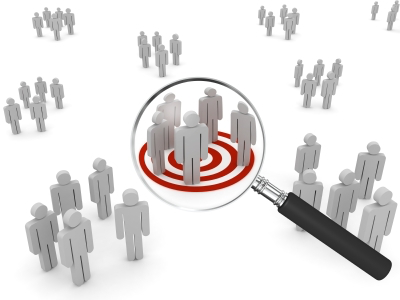
\includegraphics[width=.6\linewidth]{img/target_market.png}
\end{figure}
\begin{block}{理解用户兴趣}
一个用户属于哪个人群,是哪些广告的潜在受众。
\end{block}
\end{frame}

\begin{frame}
\frametitle{背景: User profiling}
\begin{example}{用户兴趣}
  \begin{columns}

   \pause

    \begin{column}{0.333\textwidth}
      \begin{block}{User1}
      \begin{itemize}
        \item 财经-基金
        \item 财经-股票
        \item 房产-装修
        \item ...
      \end{itemize}
      \end{block}
    \end{column}

    \pause

    \begin{column}{0.333\textwidth}
      \begin{block}{User2}
      \begin{itemize}
        \item 休闲-境外游
        \item 娱乐-综艺
        \item 休闲-摄影
        \item ...
      \end{itemize}
      \end{block}
    \end{column}

    \pause

    \begin{column}{0.333\textwidth}
    \begin{block}{User3}
      \begin{itemize}
        \item 体育-足球
        \item 体育-NBA
        \item 游戏动漫
        \item ...
      \end{itemize}
      \end{block}
    \end{column}
  \end{columns}
\end{example}

\pause

用户兴趣是多维度的 $\Rightarrow$ 标签集合 \\
标签是根据business预先设定的 

\pause

\begin{block}{}
我们要解决的实际问题:如何给用户加对应的标签?
\end{block}
\end{frame}

\section{问题与求解}

\begin{frame}
\frametitle{Overview} % Table of contents slide, comment this block out to remove it
\tableofcontents[currentsection] % Throughout your presentation, if you choose to use \section{} and \subsection{} commands, these will automatically be printed on this slide as an overview of your presentation
\end{frame}

\subsection{问题抽象}

\begin{frame}
\frametitle{问题抽象}
\begin{block}{Model and prediction}
根据给出的user feature $\mathbf{x}$,输出符合其兴趣的标签集合$\mathit{L}$.
$$\mathcal{F} : \mathcal{X} \rightarrow \mathcal{L}$$
\end{block}

\pause

\begin{block}{Model training}
To infer a $\textbf{vector-valued}$ function $\mathcal{F} : \mathcal{X} \rightarrow \mathcal{L}$ from a data set
$$\mathcal{D} = \{({\mathbf{x}}_1, {\mathbf{l}}_1), \cdots, ({\mathbf{x}}_m, {\mathbf{l}}_m)\} \in (\mathcal{X} \times \mathcal{L})$$
, where $\mathbf{x} \in \mathbb{R}^n$ and $\mathbf{l} \in {\{+1,-1\}}^L$, by minimizing \textbf{Hamming loss}:
$$\mathcal{Z}_{H} = \frac{1}{\|\mathcal{D}\|} \frac{1}{\|\mathcal{L}\|} \sum_{i=1}^{\|\mathcal{D}\|} \sum_{l=1}^{\|\mathcal{L}\|} \mathcal{I} [ \mathit{F}(\mathbf{x}_i)_l \neq \mathbf{y}_{i,l} ]$$
\end{block}
\end{frame}

%\begin{frame}
%\frametitle{Side note: why not clustering?}
%\begin{itemize}
%\item 为什么不用Clustering
%  \begin{itemize}
%    \item Cluster结果 $\neq$  pre-defined labels
%    \item 但可以作为user feature
%  \end{itemize}
%\end{itemize}
%\end{frame}

\begin{frame}
\frametitle{Multi-Label classification: Per-label bin-classification}

为了得到这个vector-valued function $\mathcal{F} : \mathcal{X} \rightarrow \mathcal{L}$, 我们为每个$\mathit{l} \in \mathcal{L}$ 都训练一个\textit{binary} classifier,预测时将判断每一个标签的结果。

* {\small \color{gray} One-versus-all implemented in LibSVM, scikit-learn, etc.} \\
* {\small \color{gray} Ad targeting往往使用per-campaign model,为每一个ad compaign训练一个二分类模型。}
\pause

优缺点:
\begin{itemize}
\item 使用已有技术 {  \color{green} \checkmark}
  \begin{itemize}
  \item LR, SVM 等二分类模型
  \end{itemize}
\item 易于验证 {  \color{green} \checkmark}
\item Not (\textit{economically}) scalable  {  \color{red} $\times$}
  \begin{itemize}
  \item num of labels: 10s $\rightarrow$ 10000s 
  \item 逐个训练低效、时间长
  \end{itemize}
\end{itemize}
\end{frame}

\begin{frame}
\frametitle{Multi-label classification: Scalable方案}
目标:
  {
    \setbeamertemplate{itemize items}[checkmark]
    \begin{itemize}
      \item 模型本身的输出就是多标签结果;
      \item 训练过程是最小化Hamming loss;
      \item Scalable.
    \end{itemize}
  }
\pause

方案:
  {
    \setbeamertemplate{itemize items}[square]
    \begin{itemize}
      \item {\color{purple} "Improved Boosting Algorithm Using Confidence-Rated Predictions", Schapire \& Singer, 1999.}
      \begin{itemize}
        \item 提出了AdaBoost.MH算法.
      \end{itemize}
      \item {\color{purple} "The return of AdaBoost.MH: multi-class Hamming trees", Kegl, 2014.}
      \begin{itemize}
        \item Factorization of base learners in AdaBoost.MH.
        \item Decision stump \& Hamming tree作为base learner.
      \end{itemize}
      \item {\color{purple} MultiBoost, http://multiboost.org}
      \begin{itemize}
        \item Open-sourced, single-machine implementations in CPP.
      \end{itemize}
    \end{itemize}
  }
\end{frame}

\subsection{Preliminary: Boosting}

\begin{frame}
\frametitle{Preliminary: Boosting}
\begin{itemize}
\item An additive model. $H(\mathbf{x}) = \sum_i^T \alpha_i h_i(\mathbf{x})$
\item 迭代的在一个 (\textit{re-})weighted sample set上去训练,
\item 通过reweighting,每次训练一个新模型去重点fix前一个模型分类错了的样本。
\end{itemize}

\begin{figure}
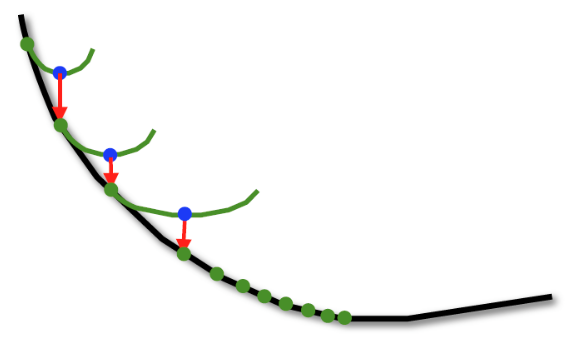
\includegraphics[width=.5\linewidth]{img/boosting.png}
\end{figure}
\end{frame}

\begin{frame}
\frametitle{Preliminary: Adaptive Boosting}

\begin{algorithm}[H]
\SetKwInOut{Input}{input}\SetKwInOut{Output}{output}
 \Input{$\mathcal{D} = (x_i, y_i) \in \{({\mathcal{R}}^n, \{-1, +1\})\}$, $T$, $\mathfrak{B}$}
 \Output{$\mathbf{H} = \Sigma_{t=1}^T{{\alpha}_t {\mathcal{B}}_t}$}
 \Begin{
   ${\mathbf{W}}_1(i) = 1/m$\;
   \For{$t \leftarrow 1, \cdots, T$}{
    ${\mathcal{B}}_t \leftarrow \mathfrak{B}(\mathcal{D}, {\mathbf{W}}_t)$\;
    Get hypothesis set: $h_t \leftarrow \mathcal{B}(\mathcal{D})$\;
    Get the base coefficient ${\alpha}_t$\;
    Update the weights: 
    $${{\mathbf{W}}_{t+1}}(i) = {{{\mathbf{W}}_{t}}(i) \exp(- {\alpha}_t y_i h_t(x_i))} / Z_t $$
    where $Z_t$ is a normalization factor\;
   }
 }
\end{algorithm}

\end{frame}

\subsection{Multi-label boosting}

\begin{frame}
\frametitle{AdaBoost.MH}
\begin{block}{}
\textbf{MH}: \textbf{M}ulti-class with \textbf{H}amming loss.
\end{block}
To produce a \textbf{vector-valued} discriminant function $\mathcal{F} : \mathcal{R}^n \rightarrow \mathcal{R}^K$ with a small \textbf{Hamming loss} $\hat{R}_H (\mathcal{F}, \mathbf{W})$ by minimizing the \textbf{weighted multi-class exponential margin-based error}
$$\hat{R}_{EXP}(\mathcal{F}, \mathbf{W}) = \frac{1}{mK} {{\Sigma}_{i=1}^m} {{\Sigma}_{l=1}^K} {\mathbf{W}_{i,l}\exp(- f_l^{(T)} y_{i,l})}$$

The weights $\mathbf{W}$:
$${\Sigma}_{i,l} \mathbf{W}_{i, l} = 1$$
\end{frame}

\begin{frame}
\frametitle{Exponential loss vs Hamming loss}
\begin{itemize}
\item Exponential loss "upper-bounds" Hamming loss.
  \begin{itemize}
    \item Minimizing exp loss is minimizing Hamming loss.
  \end{itemize}
\item Exponential loss is convex.
  \begin{itemize}
    \item Easy to optimize.
  \end{itemize}
\end{itemize}

\begin{figure}
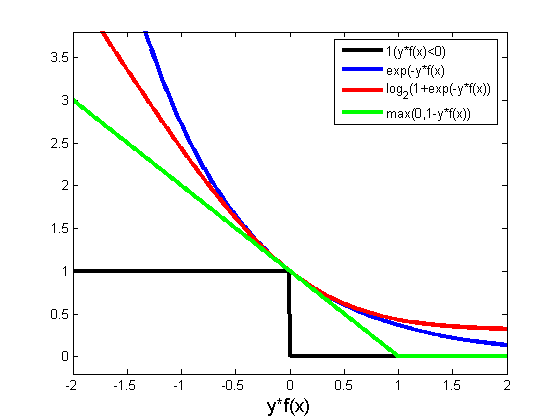
\includegraphics[width=0.6\textwidth]{img/convex-bounds.png}
\end{figure}

\end{frame}

\begin{frame}
\frametitle{AdaBoost.MH}
\begin{algorithm}[H]
\SetKwInOut{Input}{input}\SetKwInOut{Output}{output}
 \Input{$\mathcal{D} = (x_i, y_i) \in $ {\color{blue} $\{({\mathcal{R}}^n, \{-1, +1\}^K\}$ }, $T$, $\mathfrak{B}$}
 \Output{$\mathbf{H} = \Sigma_{t=1}^T{{\alpha}_t {\mathbf{B}}_t} $}
 \Begin{
   {\color{blue} ${\mathbf{W}}_1(i, l) = \frac{1}{mK}$}\;
   \For{$t \leftarrow 1, \cdots, T$}{
    Base learner and the edge: $({\mathcal{B}}_t, \gamma) \leftarrow \mathfrak{B}(\mathcal{D}, \mathbf{W}_t)$\;
    Get hypothesis set: $h_t \leftarrow \mathbf{B}(\mathcal{D})$\;
    Get the base coefficient ${\alpha}_t \leftarrow \frac{1}{2} \log \frac{1+\gamma}{1-\gamma} $\;
    Update the weights: 
    {\color{blue} $${{\mathbf{W}}_{t+1}}(i,l) = {{{\mathbf{W}}_{t}}(i,l) \exp(- {\alpha}_t y_{i,l} h_t(x_i))} / Z_t $$ }
    where $Z_t$ is a normalization factor\;
   }
 }
\end{algorithm}
\end{frame}

%% this frame highlights the coefficient \alpha to introduce ``edge'' and base learner factor.
\begin{frame}
\frametitle{AdaBoost.MH}
\begin{algorithm}[H]
\SetKwInOut{Input}{input}\SetKwInOut{Output}{output}
 \Input{$\mathcal{D} = (x_i, y_i) \in $ {\color{blue} $\{({\mathcal{R}}^n, \{-1, +1\}^K\}$ }, $T$, $\mathfrak{B}$}
 \Output{$\mathbf{H} = \Sigma_{t=1}^T{{\alpha}_t {\mathbf{B}}_t} $}
 \Begin{
   {\color{blue} ${\mathbf{W}}_1(i, l) = \frac{1}{mK}$}\;
   \For{$t \leftarrow 1, \cdots, T$}{
    Base learner and the edge: $({\mathcal{B}}_t, {\color{purple} \gamma}) \leftarrow \mathfrak{B}(\mathcal{D}, \mathbf{W}_t)$\;
    Get hypothesis set: $h_t \leftarrow \mathbf{B}(\mathcal{D})$\;
    Get the base coefficient {\color{purple} ${\alpha}_t \leftarrow \frac{1}{2} \log \frac{1+\gamma}{1-\gamma} $}\;
    Update the weights: 
    {\color{blue} $${{\mathbf{W}}_{t+1}}(i,l) = {{{\mathbf{W}}_{t}}(i,l) \exp(- {\alpha}_t y_{i,l} h_t(x_i))} / Z_t $$ }
    where $Z_t$ is a normalization factor\;
   }
 }
\end{algorithm}
\end{frame}

\begin{frame}
\frametitle{The base learner factor $\alpha$}
$$\begin{array}{c}
\hat{R}_{EXP}(\alpha, \mathbf{h}, \mathbf{W}) = \sum_{i=1}^{n} \sum_{l=1}^{K} w_{i,l} \exp(-\alpha \mathbf{h}_{i,l} y_{i,l}) \\
 = \sum_{i=1}^{n} \sum_{l=1}^{K} w_{i,l}(\mathcal{I}_+ e^{-\alpha} + \mathcal{I}_- e^{\alpha})
 \end{array},$$
$$\text{with } \mathcal{I}_+ = \mathcal{I}[y_{i,l} \mathbf{h}_{i,l} > 0], \mathcal{I}_- = \mathcal{I}[y_{i,l} \mathbf{h}_{i,l} > 0]. $$
\pause
Re-phrasing the EXP loss:
$$\begin{array}{c}
\hat{R}_{EXP}(\alpha, \mathbf{h}, \mathbf{W}) = \sum_{i=1}^{n} \sum_{l=1}^{K} w_{i,l}[ \\
  \frac{1}{2}(\mathcal{I}_+ e^{-\alpha} +\mathcal{I}_- e^{\alpha} + \mathcal{I}_+ e^{\alpha} + \mathcal{I}_- e^{-\alpha}) \\
  + \frac{1}{2}(\mathcal{I}_+ e^{-\alpha} + \mathcal{I}_- e^{\alpha} - \mathcal{I}_+ e^{\alpha} - \mathcal{I}_- e^{-\alpha})] \\
= \frac{e^\alpha + e^{-\alpha}}{2}\sum_{i=1}^{n} \sum_{l=1}^{K}\mathbf{W}_{i,j}(\mathcal{I}_+ + \mathcal{I}_-) \\
  - \frac{e^\alpha - e^{-\alpha}}{2}\sum_{i=1}^{n}\sum_{l=1}^{K}\mathbf{W}_{i,j}(\mathcal{I}_+ - \mathcal{I}_-) 
 \end{array} $$
\end{frame}

\begin{frame}
\frametitle{The base learner factor $\alpha$}
The edge $\gamma$,描述加权重之后的正确率与错误率的差。 \\
$$ \gamma(\mathbf{W}, y, \mathbf{h}) = \Sigma_{i=1}^{n} \Sigma_{l=1}^{L} \mathbf{W}_{i,l} (\mathcal{I}_+ - \mathcal{I}_-)$$
$$\text{同时,所有权重和为1: } \Sigma_{i=1}^{n} \Sigma_{l=1}^{K}\mathbf{W}_{i,l}(\mathcal{I}_+ + \mathcal{I}_-) = 1$$
\begin{block}{Exponential loss with $\gamma$:}
$$ \begin{array}{c}
\hat{R}_{EXP} = \frac{e^\alpha + e^{-\alpha}}{2}\sum_{i=1}^{n} \sum_{l=1}^{K}\mathbf{W}_{i,l}(\mathcal{I}_+ + \mathcal{I}_-) \\
 - \frac{e^\alpha - e^{-\alpha}}{2}\sum_{i=1}^{n}\sum_{l=1}^{K}\mathbf{W}_{i,l}(\mathcal{I}_+ - \mathcal{I}_-) \\
 = \frac{e^\alpha + e^{-\alpha}}{2} + \frac{e^\alpha - e^{-\alpha}}{2}\gamma.
\end{array} $$
\end{block}
\end{frame}


\begin{frame}
\frametitle{The base learner factor $\alpha$}
\begin{block}{$\alpha$ minimizing the EXP loss:}
$$\frac{\partial \hat{R}_{EXP}(\alpha, \mathbf{h}, \mathbf{W})}{\partial \alpha} = 0$$
$$\alpha = \frac{1}{2} \log \frac{1+\gamma}{1-\gamma}$$
\end{block}

\pause

\begin{block}{EXP loss becomes:}
$$\hat{R}_{EXP}(\gamma) = \sqrt{1 - \gamma^2}$$
最小化 exponential loss $\Rightarrow$ 最大化 edge。
\end{block}

\end{frame}

%% this frame highlights base learner algo to train the model
\begin{frame}
\frametitle{AdaBoost.MH}
\begin{algorithm}[H]
\SetKwInOut{Input}{input}\SetKwInOut{Output}{output}
 \Input{$\mathcal{D} = (x_i, y_i) \in $ {\color{blue} $\{({\mathcal{R}}^n, \{-1, +1\}^K\}$ }, $T$, $\mathfrak{B}$}
 \Output{$\mathbf{H} = \Sigma_{t=1}^T{{\alpha}_t {\mathbf{B}}_t} $}
 \Begin{
   {\color{blue} ${\mathbf{W}}_1(i, l) = \frac{1}{mK}$}\;
   \For{$t \leftarrow 1, \cdots, T$}{
    Base learner and the edge: {\color{purple} $({\mathcal{B}}_t, \gamma) \leftarrow \mathfrak{B}(\mathcal{D}, \mathbf{W}_t)$}\;
    Get hypothesis set: $h_t \leftarrow \mathbf{B}(\mathcal{D})$\;
    Get the base coefficient {\color{blue} ${\alpha}_t \leftarrow \frac{1}{2} \log \frac{1+\gamma}{1-\gamma} $}\;
    Update the weights: 
    {\color{blue} $${{\mathbf{W}}_{t+1}}(i,l) = {{{\mathbf{W}}_{t}}(i,l) \exp(- {\alpha}_t y_{i,l} h_t(x_i))} / Z_t $$ }
    where $Z_t$ is a normalization factor\;
   }
 }
\end{algorithm}
\end{frame}

\begin{frame}
\frametitle{Factorization of base learners}

{\color{purple} "The return of AdaBoost.MH: multi-class Hamming trees", Kegl, 2014.}
把general vector-valued function $\mathcal{B}$ 分解
\begin{itemize}
\item $\varphi(x)$: a \textit{label independent} binary classifier 
  \begin{itemize}
    \item 本质上是对\textit{feature space}做划分
  \end{itemize}
\item $\mathbf{v}$: a \textit{feature independent} vector-valued function
  \begin{itemize}
    \item 将$\varphi(x)$划分的${\pm 1}$结果cast到\textit{label space} $\{\pm 1\}^K$上
  \end{itemize}
\end{itemize}
\begin{block}{}
$$\mathcal{B}(\mathbf{x}) = \varphi(\mathbf{x}) \mathbf{v}$$
\end{block}
\end{frame}

\begin{frame}
\frametitle{Factorization of base learners}
\begin{columns}[T]
  \begin{column}{.55\textwidth}
    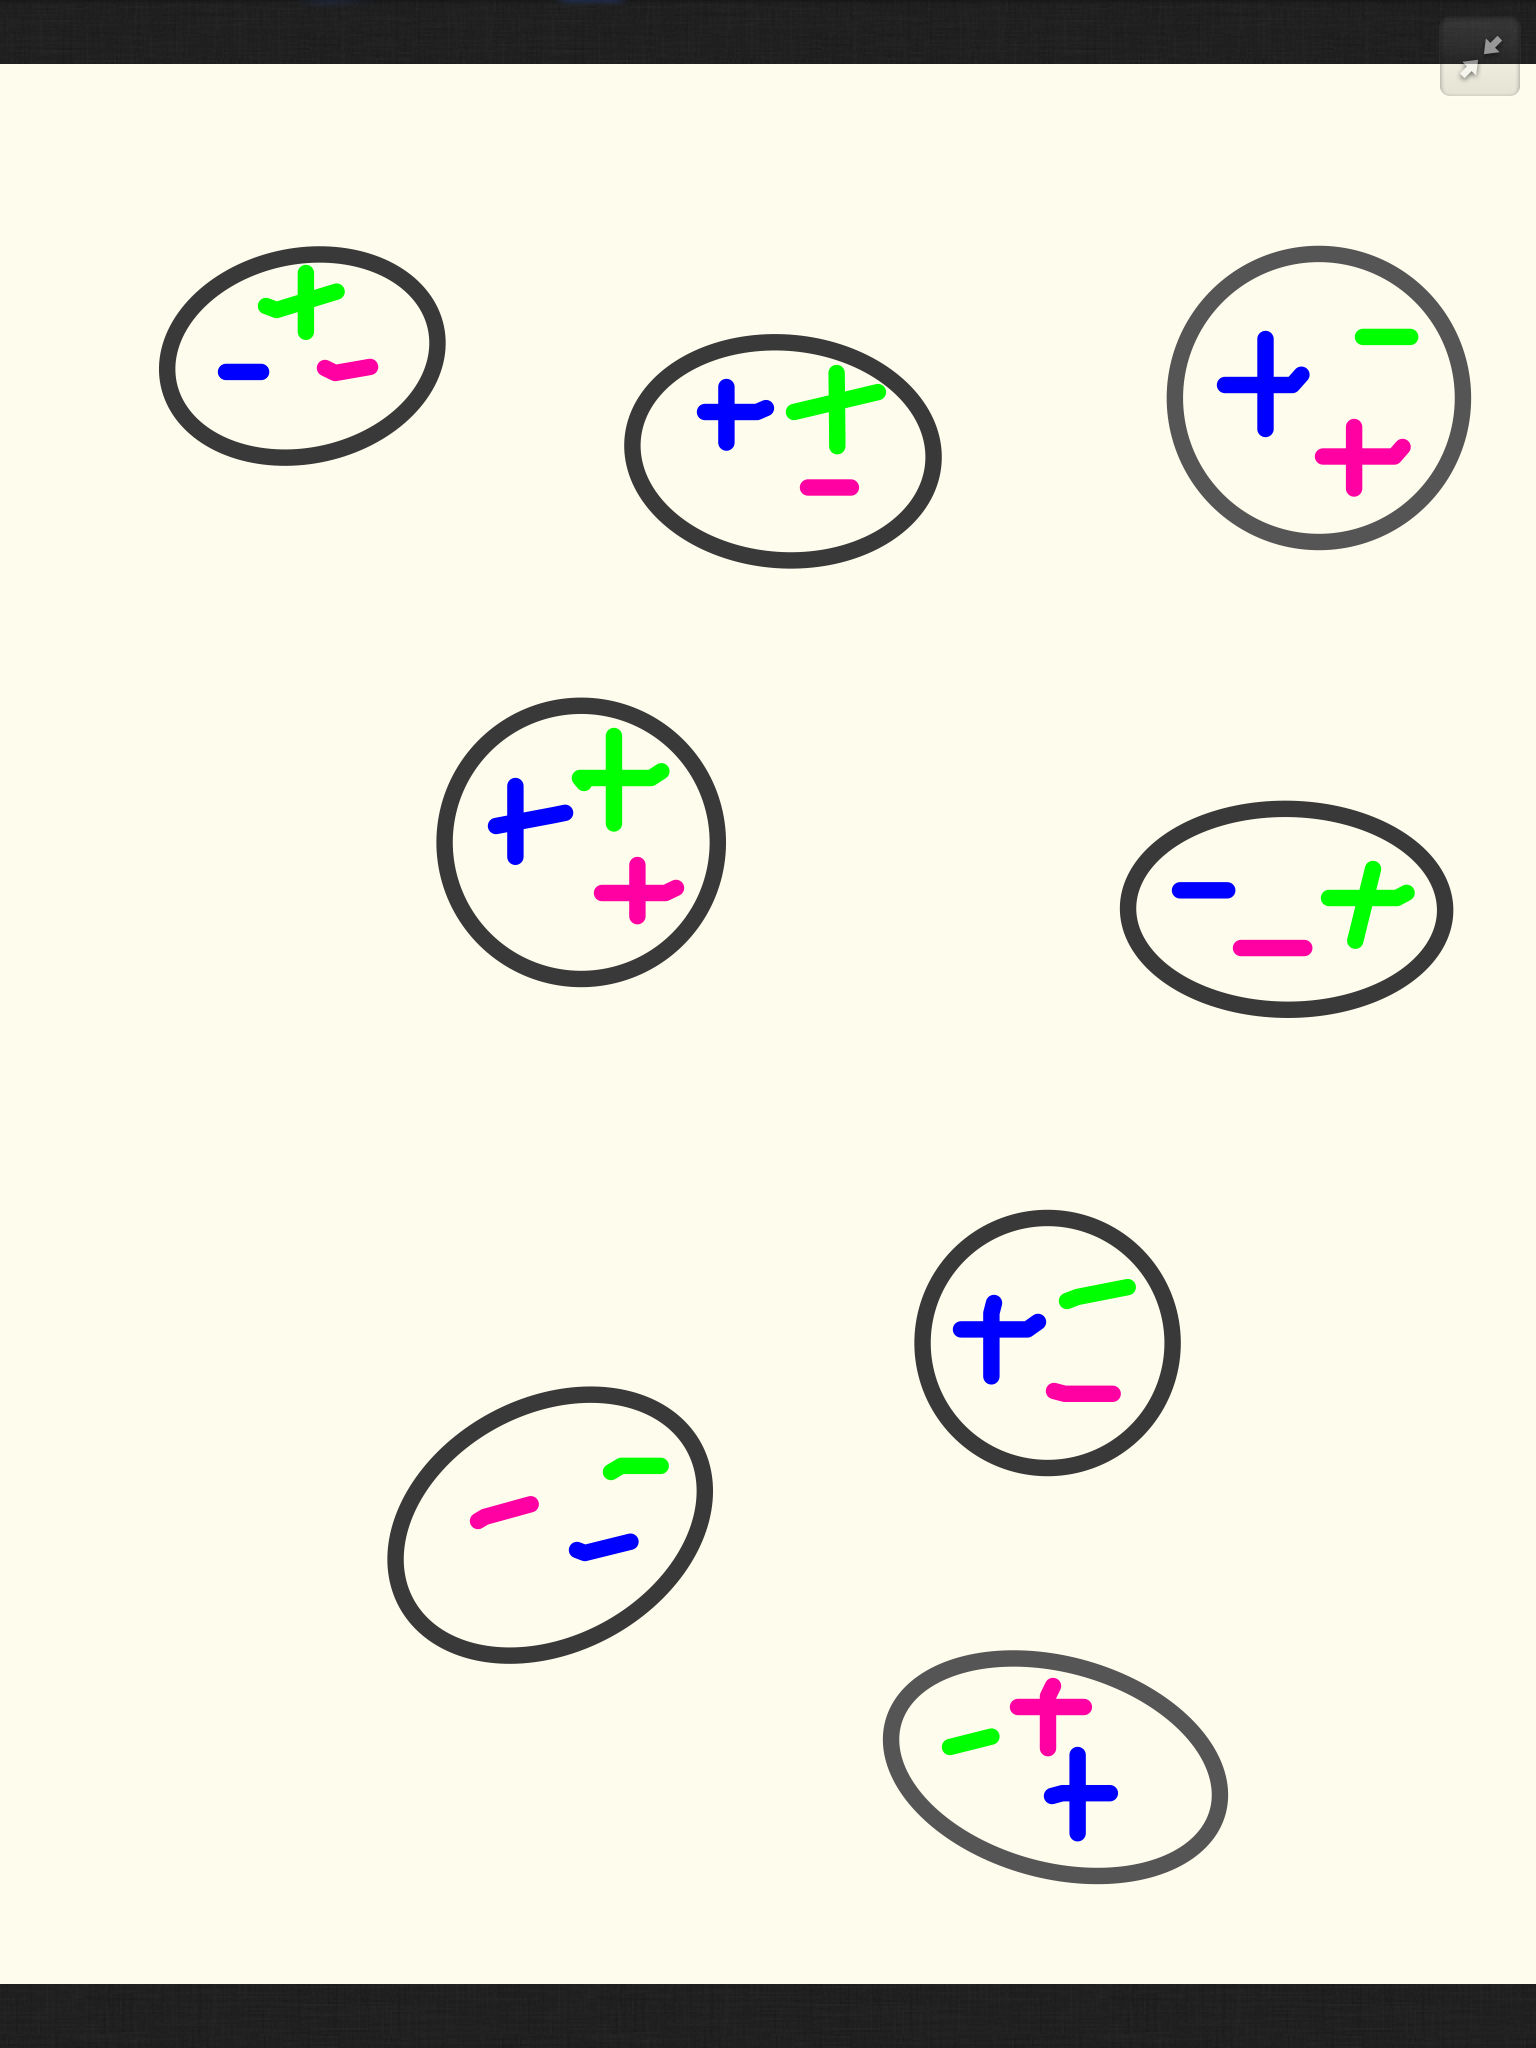
\includegraphics[width=\textwidth]{img/gbc_1.png}
  \end{column}
  \begin{column}{.45\textwidth}
    \ \\ \ \\
    有3个label的多标签分类数据集。
  \end{column}
\end{columns}
\end{frame}

\begin{frame}
\frametitle{Factorization of base learners}
\begin{columns}[T]
  \begin{column}{.55\textwidth}
    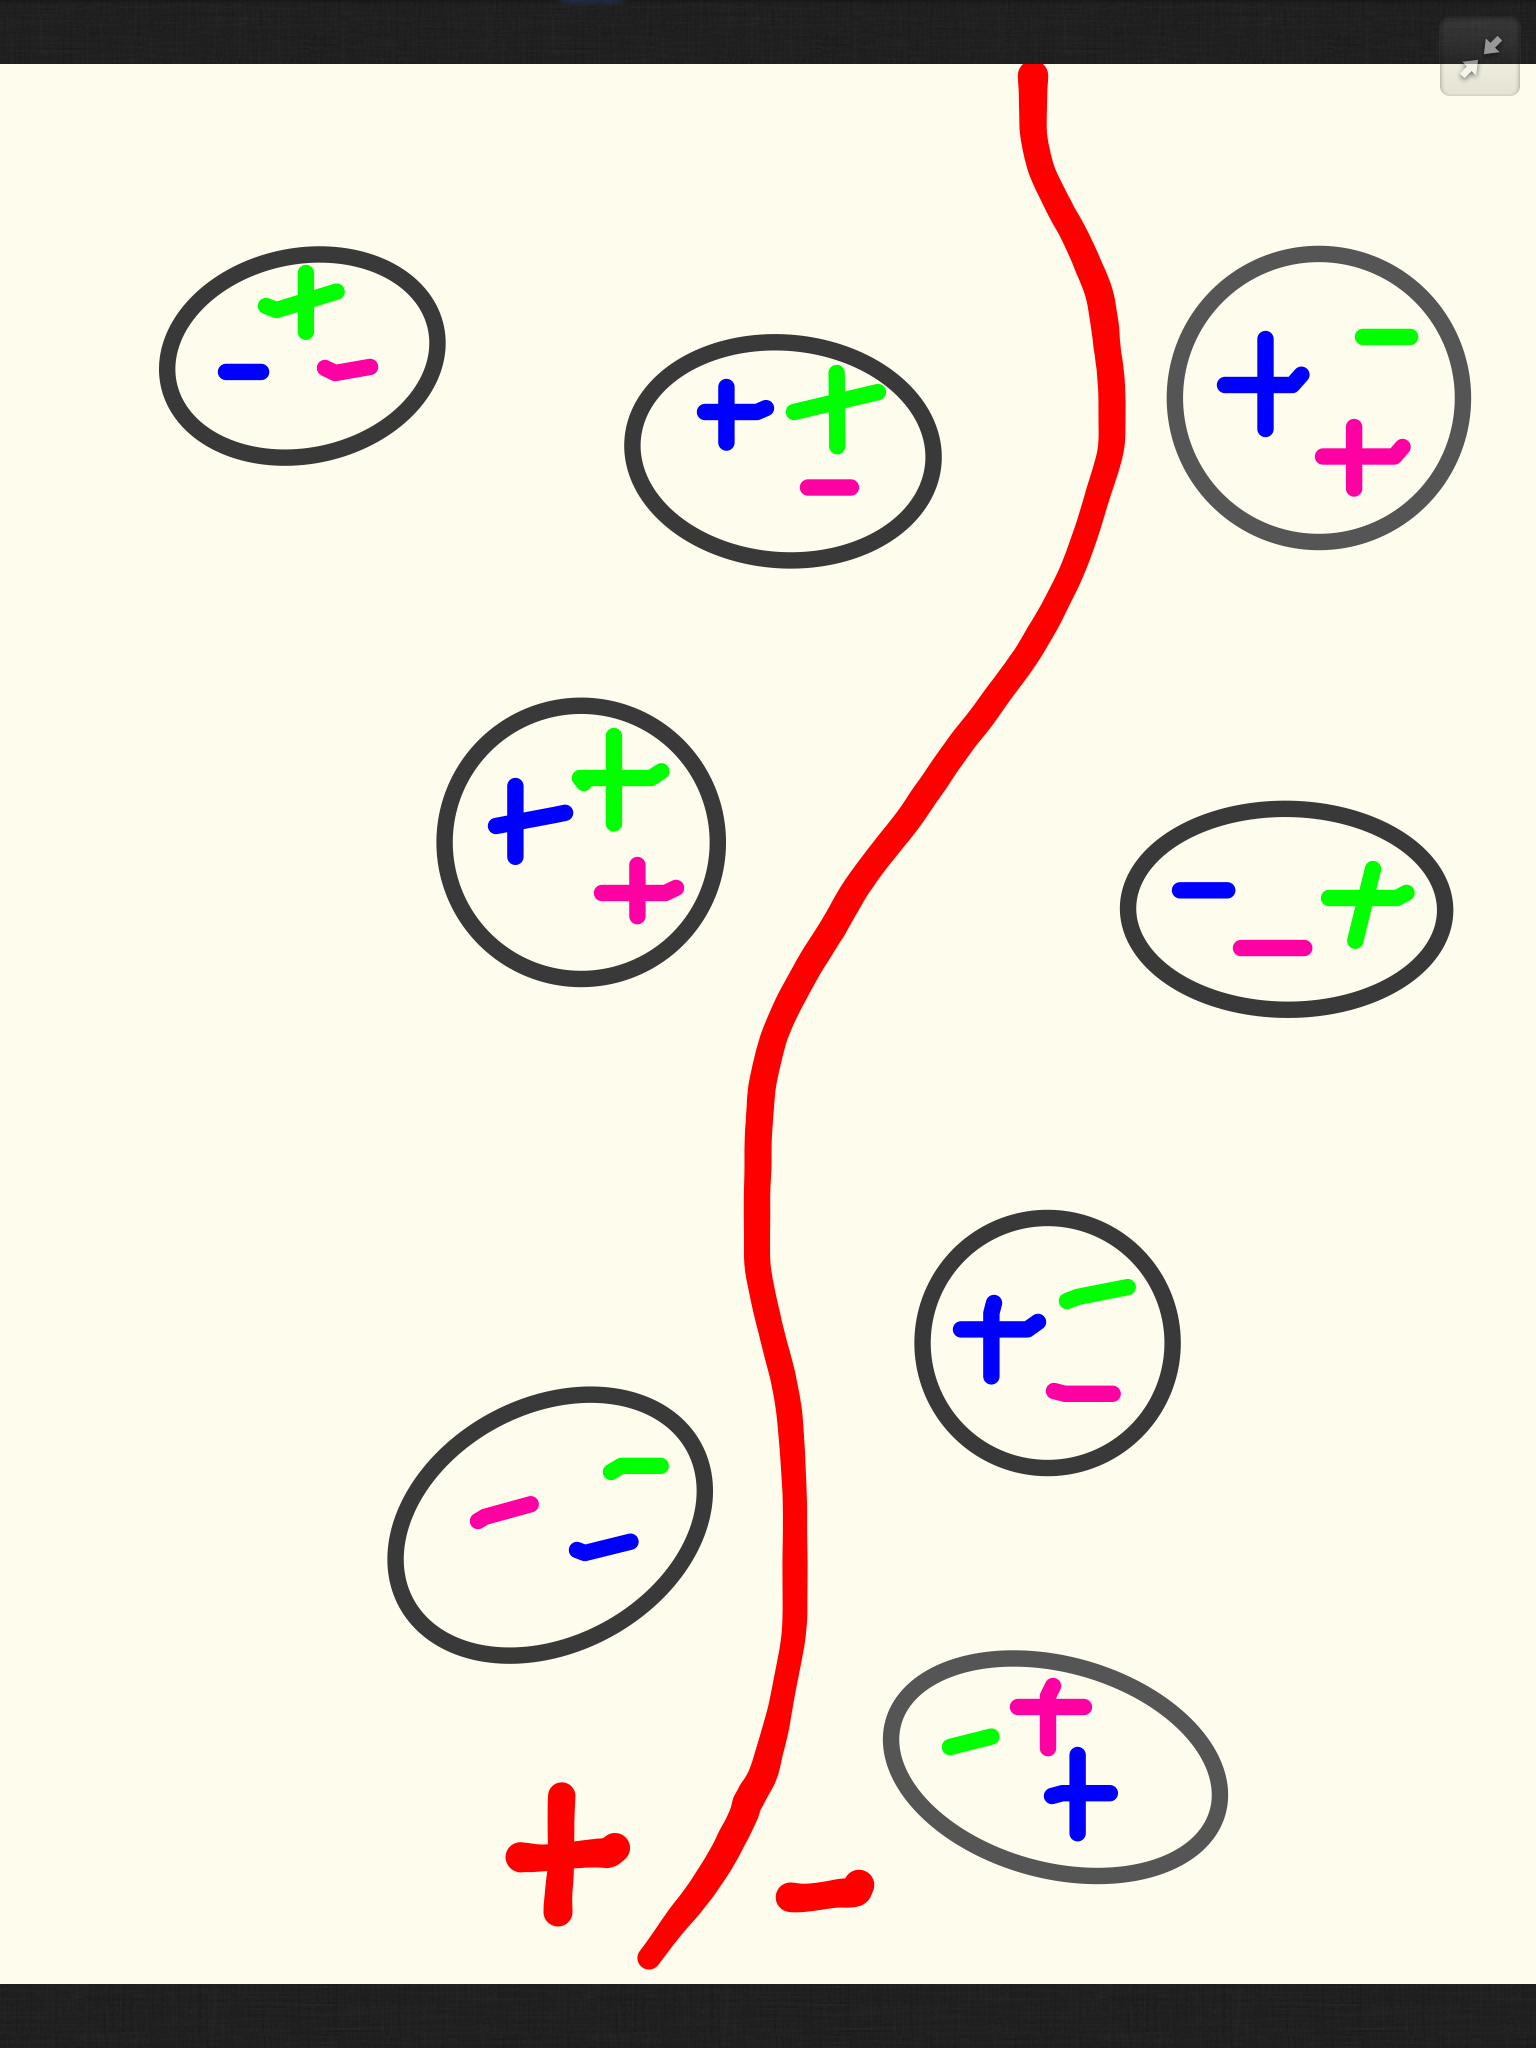
\includegraphics[width=\textwidth]{img/gbc_2.png}
  \end{column}
  \begin{column}{.45\textwidth}
    \ \\ \ \\
    $\varphi(\mathbf{x})$对\textit{feature space}做划分,将样本集分为\{+1\}和\{-1\}两部分。\\ \ \\
    $$\mathbf{v} = (v_{{\color{green} \bullet}}, v_{{\color{blue} \bullet}}, v_{{\color{magenta} \bullet}}) = (1,1,1)$$
  \end{column}
\end{columns}
\end{frame}

\begin{frame}
\frametitle{Factorization of base learners}
\begin{columns}[T]
  \begin{column}{.55\textwidth}
    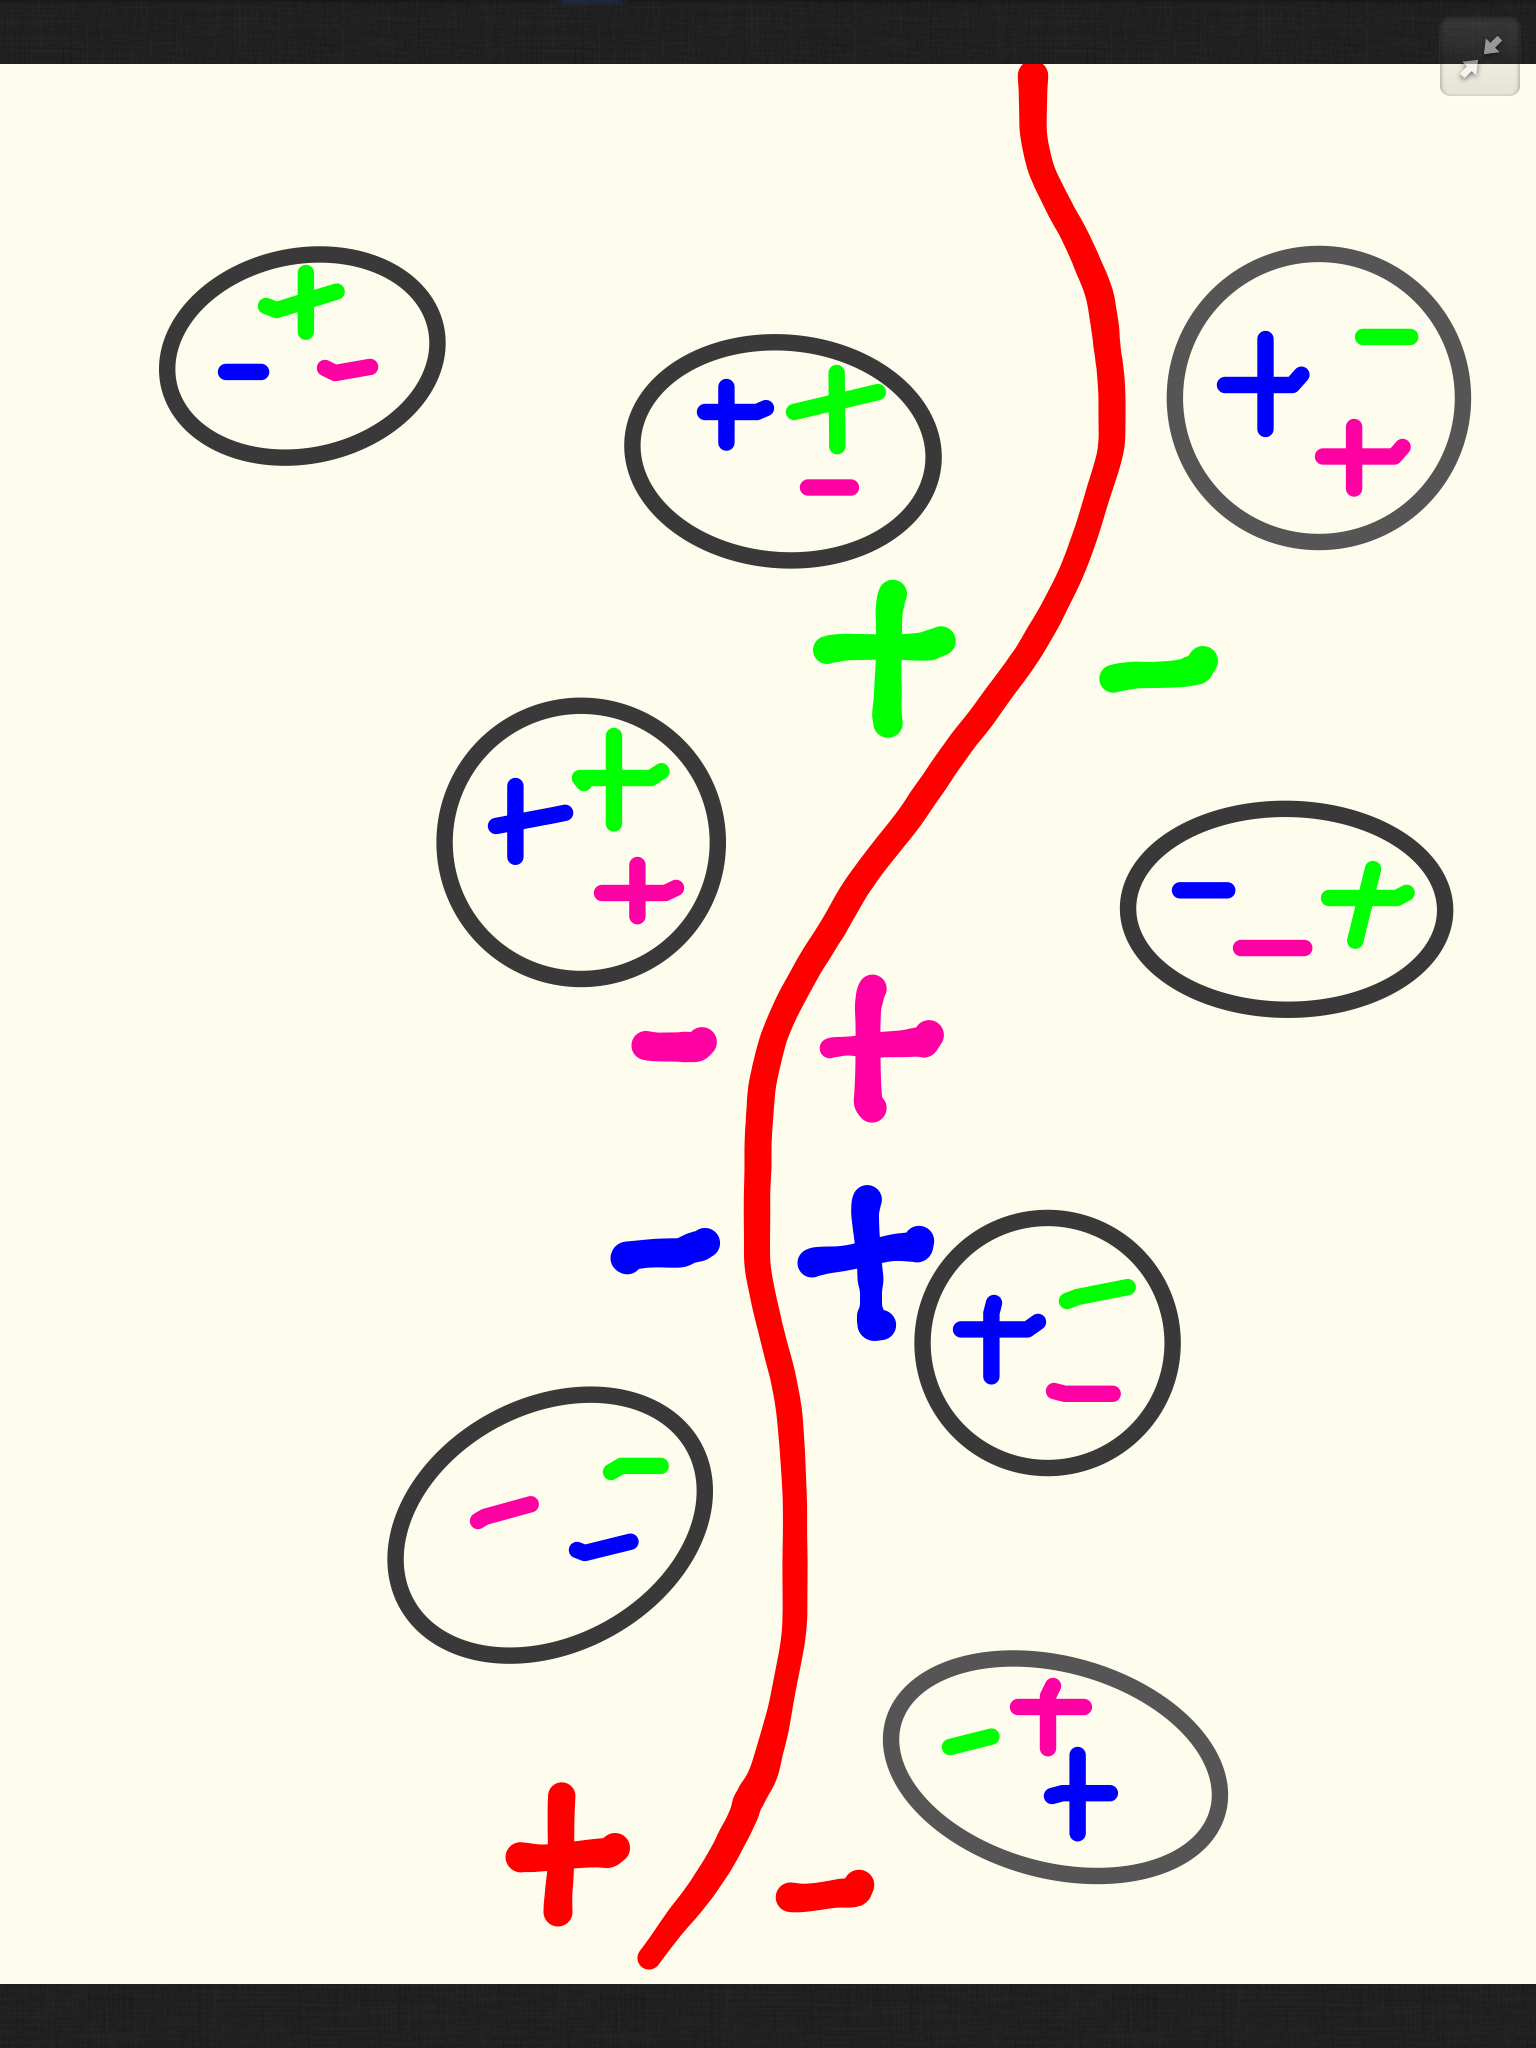
\includegraphics[width=\textwidth]{img/gbc_3.png}
  \end{column}
  \begin{column}{.45\textwidth}
    \ \\
    %根据$\varphi(\mathbf{x})$在每个label下的划分错误率,使用vote vector $\mathbf{v}$来修正结果。\\ \ \\
    %对于$\varphi(\mathbf{x})$在该label下正确率大于错误率的,如图中的{\color{green} $\bullet$},$\mathbf{v}$对应项为+1;对于正确率小于错误路的,如图中的{\color{blue} $\bullet$}和{\color{magenta} $\bullet$},$\mathbf{v}$对应项为-1。\\ \ \\
    $\varphi(\mathbf{x})$正确率高的: \\
    ${v}_{{\color{green} \bullet}} = +1,$ \\ \ \\
    $\varphi(\mathbf{x})$错误率高的,通过$\mathbf{v}$来翻转: \\
    ${v}_{{\color{blue} \bullet}} = -1,$ \\
    ${v}_{{\color{magenta} \bullet}} = -1.$
    $$\mathbf{v} = (v_{{\color{green} \bullet}}, v_{{\color{blue} \bullet}}, v_{{\color{magenta} \bullet}}) = (1,-1,-1)$$
    最终整体的在每个label上,正确率都大于错误率。 \\ \ \\
  \end{column}
\end{columns}
\end{frame}


%% this frame highlights everything we need to train the model
\begin{frame}
\frametitle{AdaBoost.MH}
\begin{algorithm}[H]
\SetKwInOut{Input}{input}\SetKwInOut{Output}{output}
 \Input{$\mathcal{D} = (x_i, y_i) \in $ {\color{blue} $\{({\mathcal{R}}^n, \{-1, +1\}^K\}$ }, $T$, $\mathfrak{B}$}
 \Output{$\mathbf{H} = \Sigma_{t=1}^T{{\alpha}_t {\mathbf{B}}_t} $}
 \Begin{
   {\color{blue} ${\mathbf{W}}_1(i, l) = \frac{1}{mK}$}\;
   \For{$t \leftarrow 1, \cdots, T$}{
    Base learner and the edge: {\color{blue} $({\mathcal{B}}_t, \gamma) \leftarrow \mathfrak{B}(\mathcal{D}, \mathbf{W}_t)$}\;
    Get hypothesis set: $h_t \leftarrow \mathbf{B}(\mathcal{D})$\;
    Get the base coefficient {\color{blue} ${\alpha}_t \leftarrow \frac{1}{2} \log \frac{1+\gamma}{1-\gamma} $}\;
    Update the weights: 
    {\color{blue} $${{\mathbf{W}}_{t+1}}(i,l) = {{{\mathbf{W}}_{t}}(i,l) \exp(- {\alpha}_t y_{i,l} h_t(x_i))} / Z_t $$ }
    where $Z_t$ is a normalization factor\;
   }
 }
\end{algorithm}
\end{frame}



%%%%%%%%%%%%%%%%%%%%%%%%%%%%%%%%%%%%%%%%%%%%%%%%%%%%%%%%%%
%
%  Model training on Apache Spark
%
%%%%%%%%%%%%%%%%%%%%%%%%%%%%%%%%%%%%%%%%%%%%%%%%%%%%%%%%%%

\section{Multiboost on Spark}

\begin{frame}
\frametitle{Overview} % Table of contents slide, comment this block out to remove it
\tableofcontents[currentsection] % Throughout your presentation, if you choose to use \section{} and \subsection{} commands, these will automatically be printed on this slide as an overview of your presentation
\end{frame}

\subsection{Strong learner on Apache Spark}

\begin{frame}
\frametitle{Strong learner on Apache Spark}
\begin{itemize}
\item Spark的driver program中实现算法逻辑
\item Base learner类型作为类型参数
  \begin{itemize}
    \item 不同base learner可替换,pluggable
    \item Base learner的training逻辑与strong learner解耦合
  \end{itemize}
\end{itemize}
{ \small
\href{https://github.com/BaiGang/spark_multiboost/blob/master/src/main/scala/org/apache/spark/mllib/classification/multilabel/stronglearners/AdaBoostMH.scala}{https://github.com/...../.../stronglearners/AdaBoostMH.scala}
}
\begin{figure}
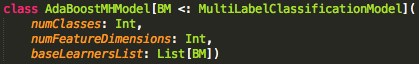
\includegraphics[scale=0.5,left]{img/adbm_model_spark.png} \\
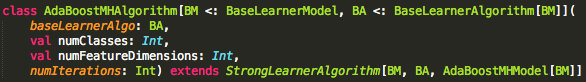
\includegraphics[scale=0.5,left]{img/adbm_algo_spark.png} \\
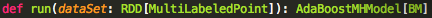
\includegraphics[scale=0.5,left]{img/adbm_run.png}
\end{figure}
\end{frame}

\begin{frame}
\frametitle{AdaBoost.MH on Apache Spark}
迭代过程:
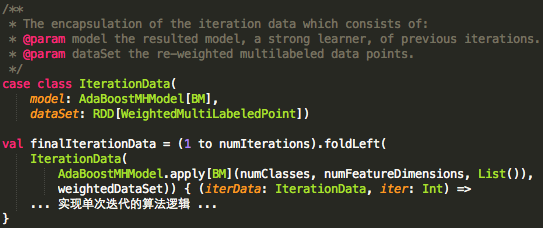
\includegraphics[scale=0.5,left]{img/iteration.png}
\end{frame}

\begin{frame}
\frametitle{AdaBoost.MH on Apache Spark}
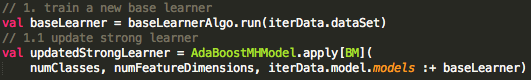
\includegraphics[scale=0.5,left]{img/a1_train_base.png} \\
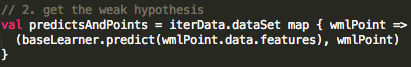
\includegraphics[scale=0.5,left]{img/a2_hypoth.png} \\
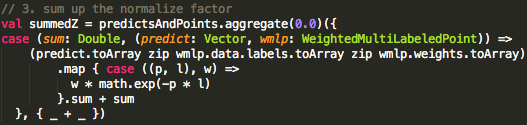
\includegraphics[scale=0.5,left]{img/a3_sumz.png} \\
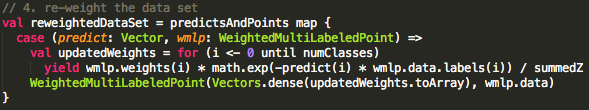
\includegraphics[scale=0.5,left]{img/a4_reweighting.png} \\
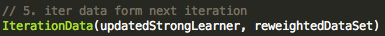
\includegraphics[scale=0.5,left]{img/a5_nextiter.png} 
\end{frame}

\subsection{Base learner on Apache Spark}

\begin{frame}
\frametitle{Base learner on Apache Spark}
最核心的内容是实现 {\color{blue} \texttt{baseLearnerAlgo.run(iterData.dataSet)}}。 \\ \ \\
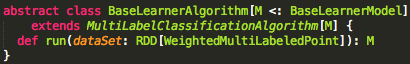
\includegraphics[scale=0.5,left]{img/base_algo.png}
\end{frame}

\begin{frame}
\frametitle{Base learners}
{
  \setbeamertemplate{itemize items}[checkmark]
  \begin{itemize}
    \item Decision stump: 一个只有一个结点的决策树
       $$ \varphi_{j,b}(\mathbf{x}) = \left\{
            \begin{array}{l l}
              1 & \quad \text{if } \mathbf{x}_j \geq b, \\
             -1 & \quad \text{otherwise.}
            \end{array} \right.$$
    \item Hamming tree: Decision stump作为结点的决策树
    \item Generalized bin-classifier方案
      \begin{itemize}
        \item $\varphi(x)$使用任意二分类模型,与$\mathbf{v}$一起来最大化class-wise edge/最小化exp loss。
      \end{itemize}
  \end{itemize}
}
\end{frame}

\begin{frame}
\frametitle{Decision stump model}
  \begin{itemize}
    \item 寻找最优划分来maximize "discriminability": $(j*,b*) = \argmax_{j,b} \sum_{l}\| \gamma_l \|$
    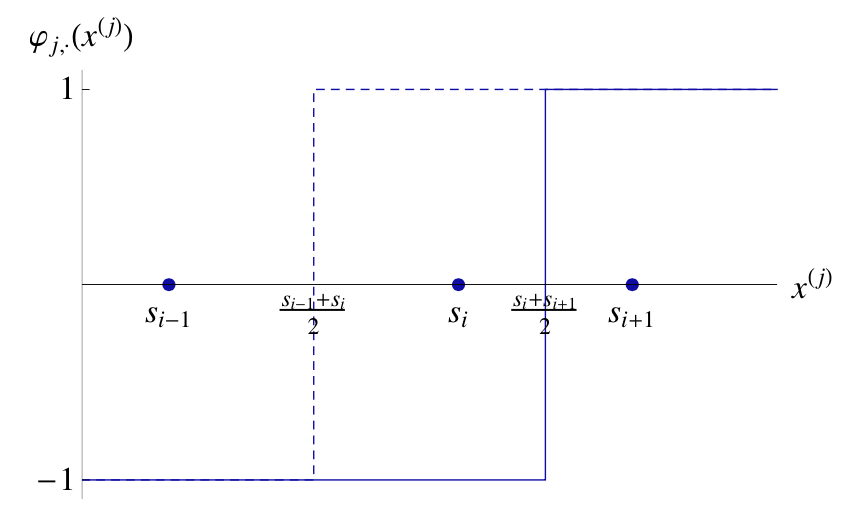
\includegraphics[width=0.6\textwidth]{img/ds_split.png}
    \begin{itemize}
      \item $\text{If } y_{i,l}=1, \gamma_l -= 2w_{il}; \text{Or } y_{i,l}=-1, \gamma_l += 2w_{i,l}.$
    \end{itemize}
    \item 单机版:$\mathbf{x}_j$排序复杂度$\mathcal{O}(m\log(m))$,搜索的过程$\mathcal{O}(m)$,总的$\mathcal{O}(nm\log(m))$
    \item Spark: {\color{blue} \texttt{flatMap} $\rightarrow$ \texttt{reduceByKey}}
  \end{itemize}
\end{frame}

\begin{frame}
\frametitle{Decision stump on Spark: Implementation}
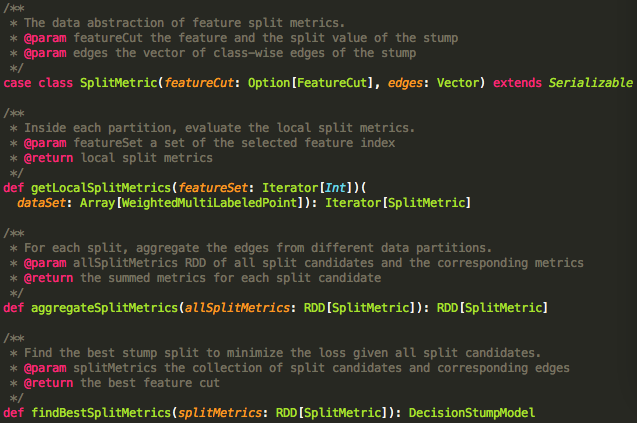
\includegraphics[width=0.99\textwidth]{img/decision_stump_spark.png}
\end{frame}

\begin{frame}
\frametitle{Decision stump on Spark: Results}
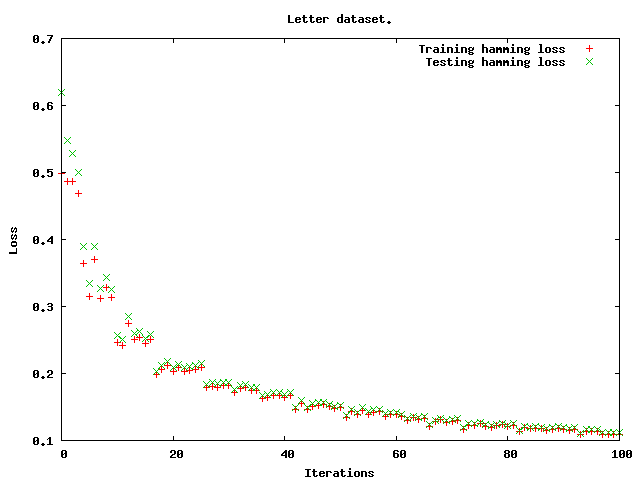
\includegraphics[width=0.45\textwidth]{img/letter.png} \ 
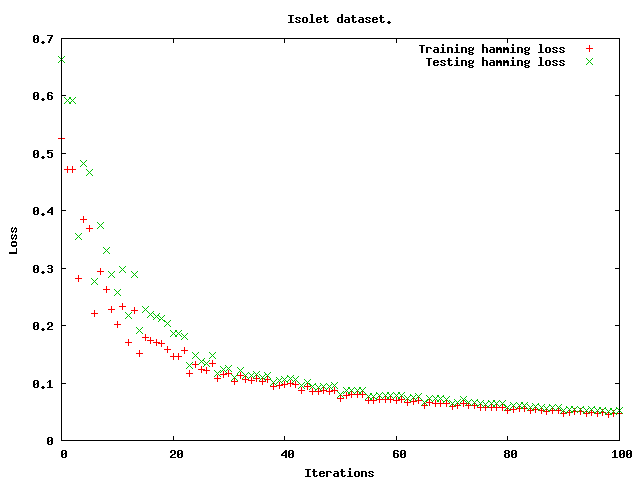
\includegraphics[width=0.45\textwidth]{img/isolet.png} \\
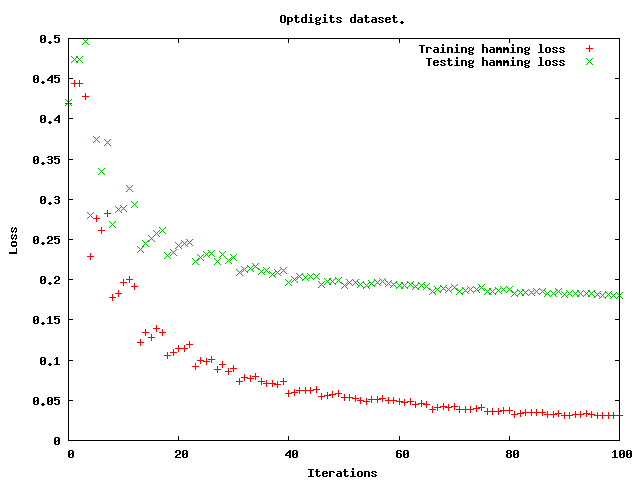
\includegraphics[width=0.45\textwidth]{img/optdigits.png} \ 
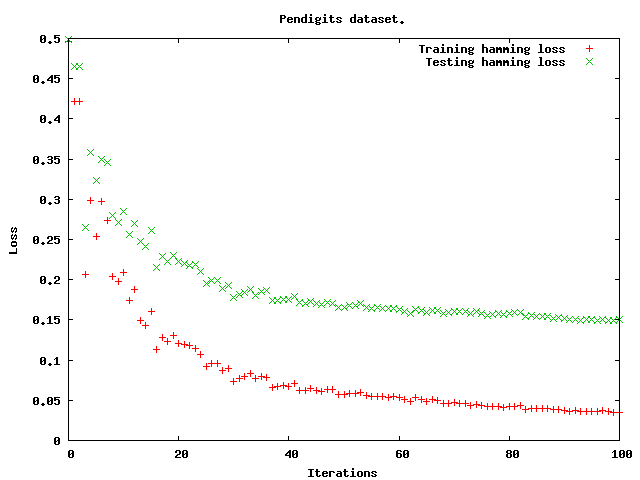
\includegraphics[width=0.45\textwidth]{img/pendigits.png} \\
{ \small
    "letter", "isolet", "optdigits" and "pendigits" from UCI dataset \\
    \href{http://archive.ics.uci.edu/ml/datasets.html}{http://archive.ics.uci.edu/ml/datasets.html}
}
\end{frame}

\begin{frame}
\frametitle{Decision stump on Spark: Performance}
{ \small
n: 150k+, $\|\mathbf{D}\|$ = 342926; run on 500 RDD partitions, 150 executors.\\
}
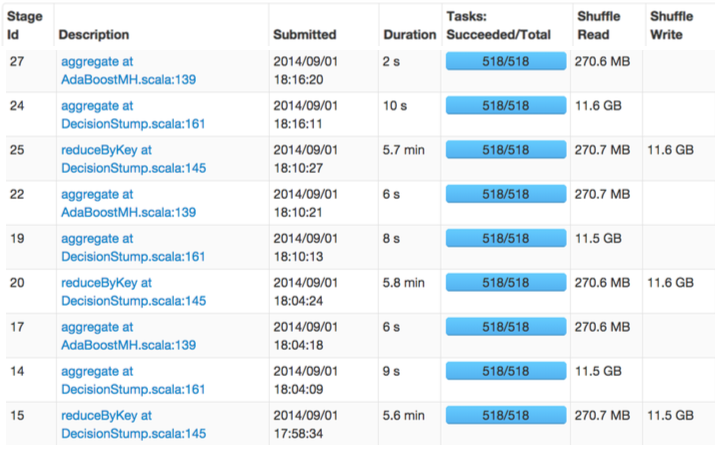
\includegraphics[width=0.9\textwidth]{img/ds_perf.png}
\end{frame}

\subsection{Base learner: generalized binary classifier with vote vector}

\begin{frame}
\frametitle{Base learner: generalized binary classifier with vote vector}
\begin{itemize}
\item Decision stump的问题
  \begin{itemize}
    \item 是非常弱的二分类模型
    \item Decision stump模型训练的数据传输量很大
    \item Tree-based模型,并不适合高维稀疏数据
  \end{itemize}
\end{itemize}

\pause

\begin{block}{}
我们需要一个更强的、更易于训练并且适应高维稀疏数据的$\varphi(\cdot)$,来对\textit{feature space}做二元划分。
\end{block}
\end{frame}

%\begin{frame}
%\frametitle{Generalized binary classifier as $\varphi(\bullet)$}
%\begin{itemize}
%\item $\varphi(x)$使用任意二分类模型,以最大化class-wise edge/最小化exp loss为目标
%\item $\mathbf{v}$与$\varphi(x)$交替求解
%\end{itemize}
%\begin{algorithm}[H]
%\SetKwInOut{Input}{input}\SetKwInOut{Output}{output}
% \Input{$\mathbf{W}, \mathcal{D}, N$}
% \Output{$\varphi(\cdot), \mathbf{v}$}
% \Begin{
%   $\mathbf{v} = vec(1, 1, \cdots 1)$\;
%   \For{$i \leftarrow 1, \cdots, N$}{
%    $\varphi(\cdot)$: $\varphi(\cdot) = \argmin_{\hat{\varphi}(\cdot)} \hat{R}_{EXP}(\mathbf{h}(\varphi(\mathbf(x)), \mathbf{v}) \mathbf{W})$\;
%    $\mathbf{v}$: $\mathbf{v} = \argmin_{\hat{\mathbf{v}}} \hat{R}_{EXP}(\mathbf{h}(\varphi(\mathbf(x)), \mathbf{v}) \mathbf{W})$\;
%   }
%   $\varphi(\cdot), \mathbf{v}$
% }
% \end{algorithm}
%
%$(\varphi*(\cdot),\mathbf{v}*) = \argmin_{\varphi(\cdot), \mathbf{v}} \hat{R}_{EXP}$
%\end{frame}

\begin{frame}
\frametitle{Generalized binary $\varphi$ on Apache Spark}
\begin{itemize}
\item 使用spark.mllib.classification中已有的model/algorithm
\begin{itemize}
  \item SVM, LR with GradientDescent, LBFGS.
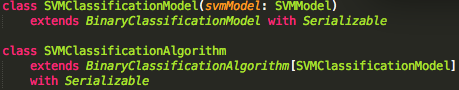
\includegraphics[scale=0.5]{img/svm_bin.png}
\end{itemize}
\item Boosting机制,只要base learner比random guess好,整体就是收敛的
  \begin{itemize}
    \item 通过vote vector $\mathbf{v}$ 来保证每个label上的错误率小于0.5。
  \end{itemize}
\item 将$\mathbf{D} \in \{(\mathcal{R}^n, {\color{blue} \{\pm1\}^K } )\}$转化成$\mathbf{D}' \in \{(\mathcal{R}^n, { \color{blue} \{\pm1\} } )\}$,作为binary classification的数据集
  \begin{itemize}
    \item 使用$\{\pm1\}^K$中的一个维度作为1维label的取值
    \item $\mathbf{D} \Rightarrow \mathbf{D}'$是需要进一步考虑的部分 *TODO
  \end{itemize}
\end{itemize}
\end{frame}

\section{后续工作}

\begin{frame}
\frametitle{后续工作}

\begin{itemize}
\item 训练$\varphi(\cdot)$时,如何转换数据集$\mathbf{D} \Rightarrow \mathbf{D}'$,使得base learner的效果最好
\item 使用LR、SVM作为$\varphi(\cdot)$,其loss与edge-maximizing目标一致性需要理论证明
\item $\star$ 现有实现基于Spark 1.1.x, 应用新的spark ml interface
\item $\star \star \star$ 定义新的判别模型$\varphi(\cdot)$,实现exp loss对应的梯度计算$\frac{\partial \hat{R}_{EXP}}{\partial \varphi(\cdot)}$,优化求解模型参数
\end{itemize}

\begin{block}{欢迎fork \& pull request!}
\url{https://github.com/baigang/spark_multiboost}
\end{block}

\end{frame}

\end{document} 
